\chapter{Data manipulation and Pandas library}

In this chapter, our goal is to explore the world of data manipulation.
We explain what data structures are usually used and what do the common operations on them look like.
We will need the information in the next chapters when defining the Abstract Interpretation framework for these data
structures.
We show the concepts on Pandas and discuss what Pandas does differently.
% todo what about the types

\section{Data structures} %============================================================================================%

When we talk about data structure, we usually define it as a way of organizing data in the computer memory.
However, there are two concepts to distinguish - the interface and the implementation.

The interface is a set of operations that we are allowed to do with the data structure as a users.
Good example of a data structure interface can be an Array, List, Dictionary or a Heap.
Implementation on the other hand is how the data structure works under the hood to provide the interface promised.
To give an example of an implementation of a data structure I mention a binary tree, n-ary heap or a linked list.

In this chapter, when talking about data structures, we omit the implementation details, and we focus only on the
interface of the data structure i.e.\ what operations are provided.
Also, we assume the existence of primitive data types such as integers, floating-point numbers, strings etc.

\begin{defn}[List interface]
    \textbf{List} interface is a set of methods for random access, appending, inserting, updating and removing elements
    from a collection.
    All operations use numeric zero-based indexing.
\end{defn}

\begin{defn}[Dictionary interface]
    \textbf{Dictionary} interface supports accessing, adding, replacing or removing elements from a collection.
    All operations use key-based indexing.
\end{defn}

\subsection{Series}

The first and the simplest data structure is usually called Series.
In its simplest form it is a one-dimensional data structure holding data of some primitive data type.
It supports a List interface, so random access based on integer indexing is supported as well as adding, removing and
modifying items.

The Listing~\ref{lst:series_basics} shows basic work with the Series data structure in Pandas.

\begin{lstlisting}[caption=Working with Series in Pandas, label={lst:series_basics}, captionpos=b]
import pandas as pd
# Creating series
series = pd.Series([1, 1, 2, 3, 5, 8])

# Adding an element
series[6] = 13

# Removing an element at index 0
series.drop(0, inplace=True)

# Replacing an element
series[1] = 100
\end{lstlisting}

There can also be an index associated with the Series.
The index is a set of distinct values of any primitive type (usually a string or a time) associated with the values of
the Series.
It expands the interface of a Series with a Dictionary interface.
Consequently, the items can be accessed using the values in the index.
Another usual feature of a Series is an optional label describing the data.
Listing~\ref{lst:series_index} shows how the work with index works in Pandas.

\begin{lstlisting}[caption=Index on a Series, label={lst:series_index}, captionpos=b]
import pandas as pd

# Creating series with index
data = [1, 2, 3, 4]
index = ["first", "second", "third", "fourth"]
series = pd.Series(data=data, index=index)

# Accessing based on index
print(series["second"]) # Prints 2

# Adding based on index
series["fifth"] = 5

# Removing based on index
series.drop("fifth", inplace=True)

\end{lstlisting}

Contrary to what we said, Series in Pandas is a heterogeneous data structure - it is able to hold values of different
types together.
So the code showed in Listing~\ref{lst:series_heterogeneous} is completely valid Pandas code.

\begin{lstlisting}[caption=Heterogenous Series, label={lst:series_heterogeneous}, captionpos=b]
import pandas as pd

# Create a series of values with different types
series = pd.Series([0, True, "two", "three", 4])
\end{lstlisting}

The explanatory visualization of a Series can be found in the Figure~\ref{fig:series_schema}

\begin{figure}[H]
    \caption{Schema of a Series}
    \label{fig:series_schema}
    \centering
    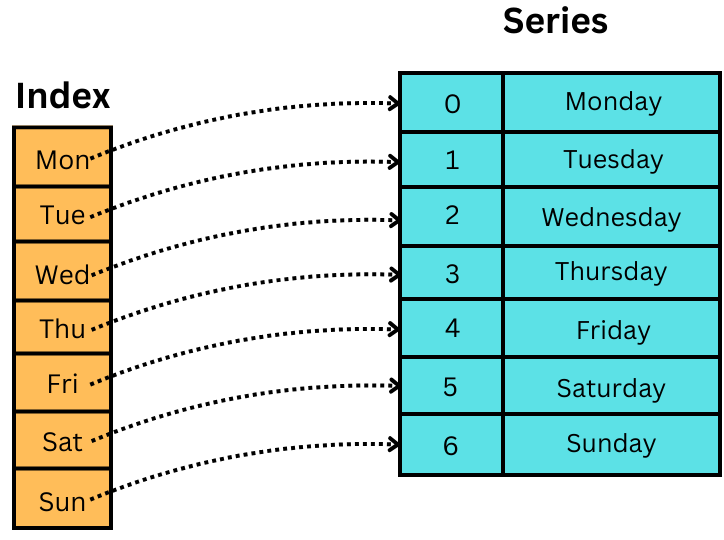
\includegraphics[scale=0.4]{img/Series}
\end{figure}

\subsection{Dataframe} % todo csv, excel, ...

Dataframe is a two-dimensional tabular data structure.
A good way to look at a Dataframe is to see it as a Dictionary, where the keys are names of a columns of a table
and values are Series representing the columns themselves.
This also means that the Dataframe supports indexing of columns based on column names and integer-based indexing of rows.
Listing \ref{lst:dataframe_basics} shows basic work with the Dataframe in Pandas.

\begin{lstlisting}[caption=Working with Dataframe in Pandas, label={lst:dataframe_basics}, captionpos=b]
import pandas as pd

# Create a dataframe from a map of columns
data = {"column1": [1, 2, 3], "column2": ['a', 'b', 'c']}
dataframe = pd.DataFrame(data)

# Add a new row
dataframe.loc[3] = [4, 'd']

# Add a new column
dataframe['column3'] = [True, False, True, False]

# Replace a value
dataframe.at[1, 'column3'] = True
\end{lstlisting}

The Dataframe can also have an index associated with the rows of Series.
Consequently, the Dataframe supports Dictionary interface on both rows and columns.
Adding of new columns and rows is also supported.
The listing~\ref{lst:dataframe_index} shows how we can use indexes when working with Dataframes in Pandas.

\begin{lstlisting}[caption=Index on a Dataframe, label={lst:dataframe_index}, captionpos=b]
import pandas as pd

# Create a dataframe with index
dataframe = pd.DataFrame({
    'A': [1, 2, 3],
    'B': [4, 5, 6],
    'C': [7, 8, 9]
}, index=['x', 'y', 'z'])

# Access elements via index
print(dataframe.at['x', 'A']) # Prints 1

# Change value using index
dataframe.at['z', 'C'] = -9
\end{lstlisting}

The explanatory visualization of a Dataframe can be found in the Figure~\ref{fig:dataframe_schema}

\begin{figure}[H]
    \caption{Schema of a Dataframe}
    \label{fig:dataframe_schema}
    \centering
    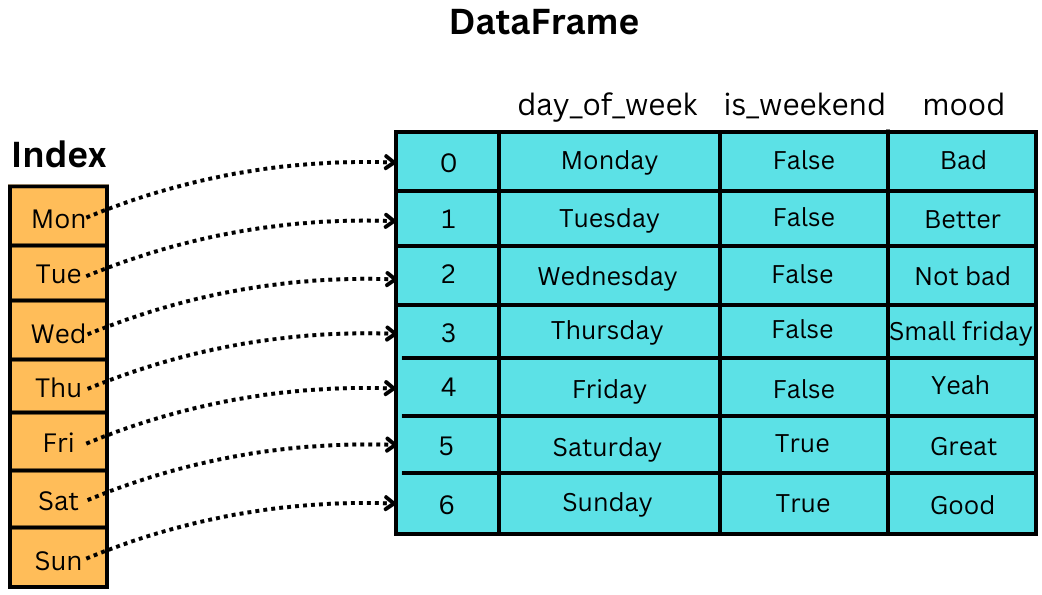
\includegraphics[scale=0.4]{img/Dataframe}
\end{figure}


\section{Common operations} %==========================================================================================%

To actually manipulate the data into some useful form, we need operations that are more powerful than just indexing and
adding and removing elements.
The operations that are commonly used in data manipulation were greatly influenced by the operations on relational
databases and the SQL language.
However, they are usually more flexible and customizable. % todo explain more

\subsection{Relational operations}

All well-known SQL relational databases support the following operations:
\texttt{SELECT, GROUP BY, HAVING, WHERE, JOIN, ORDER BY, AS}.
All these operations are also (usually under a different name) present in the data manipulation libraries as well.
We go through these operations and discuss their counterparts in Pandas.

\paragraph{SELECT} \leavevmode \\

The SELECT statement in SQL serves to select a specific subset of columns of a table.
In Pandas the square-brackets operator is used for that purpose.
As listing~\ref{lst:pandas_select} shows, the operator can return a Series or a Dataframe depending on whether
the argument is just a string or a list of strings.

\begin{lstlisting}[caption=Select in Pandas, label={lst:pandas_select}, captionpos=b]
dataframe = ... # initial dataframe

# Select a subset of columns (returns a dataframe)
subset = dataframe[["column1", "column3"]]

# Select one column (returns a series)
column = dataframe["column2"]
\end{lstlisting}

Alternatively, the filter function can be also used for this purpose.
The important information for us will be that the operation returns a Dataframe with a different column structure
than the input Dataframe - it removes non-specified columns.

The SELECT statement in SQL can also do more than just selecting a subset of columns.
It can also apply aggregating function when used with group by.
This option is covered later when we talk about the GROUP BY operation.

\paragraph{WHERE} \leavevmode \\

The WHERE statement in SQL filters out the rows that do not match a given predicate.
In this case Pandas was also able to make use of the square-brackets operator.
This time the operator accepts a Series of bool values and uses just the columns of a Dataframe with index same as
some True value in the Series.
The Series of bools is usually (but not necessarily) created using vectorized operations.
The listing~\ref{lst:pandas_where} shows the usage.

\begin{lstlisting}[caption=Where in Pandas, label={lst:pandas_where}, captionpos=b]
dataframe = ... # initial dataframe

# Select just rows where the "age" column is at least 18
adults = dataframe[dataframe["age"] >= 18]
\end{lstlisting}

The important information for us will be that the result of this operation is a Dataframe with the same column structure.

\paragraph{AS} \leavevmode \\

The AS keyword is used to rename a specific column.
Pandas also has this feature, although it is named differently.
The function is called rename, and it accepts a mapping from old column names to new column names.
The listing~\ref{lst:pandas_as} shows how the rename function can be used.

\begin{lstlisting}[caption=As in Pandas, label={lst:pandas_as}, captionpos=b]
dataframe = ... # initial dataframe

# Rename some of the columns
renamed_dataframe = dataframe.rename(
    columns={"column1": "col1", "column2": "col2"}
)
\end{lstlisting}

\paragraph{ORDER BY} \leavevmode \\

ORDER BY is used to sort the data by some column.
Pandas can do the same using the sort\_values function.
The example usage can be seen in the listing~\ref{lst:pandas_orderby}

\begin{lstlisting}[caption=Order by in Pandas, label={lst:pandas_orderby}, captionpos=b]
dataframe = ... # initial dataframe

# Order the dataframe rows by the values of column
# 'surname' in the ascending order
sorted = dataframe.sort_values(by=["surname"], ascending=True)
\end{lstlisting}

Note that the operation does not change the column structure of the Dataframe.

\paragraph{JOIN} \leavevmode \\

Join operation is used to combine rows from two tables based on some related columns.
There are four types of join - inner, left, right and outer.
Inner join returns rows that have matching rows in both tables.
Left join returns all rows from the left table and all matched rows from the right table.
Right join returns all rows from the right table and all matched rows from the left table.
And outer join returns rows where there is a match in either of the tables.

Pandas has a function called merge for this purpose.
It accepts two Dataframes and returns their corresponding join.
Besides the already mentioned joins, merge also supports a cross join, which is essentially a cartesian product of
two sets of rows.
The listing~\ref{lst:pandas_join} shows how the merge function can be used as well as what parameters does the
function accept.

\begin{lstlisting}[caption=Join in Pandas, label={lst:pandas_join}, captionpos=b]
dataframe1 = ... # 1st initial dataframe
dataframe2 = ... # 2nd initial dataframe

inner = pd.merge(
    dataframe1, dataframe2, how="inner",
    left_on="left_key", right_on="right_key")
left = pd.merge(
    dataframe1, dataframe2, how="left", on="common_key")
right = pd.merge(
    dataframe1, dataframe2, how="right", on="common_key")
outer = pd.merge(
    dataframe1, dataframe2, how="outer",
    left_on="left_key", right_on="right_key"
cross = pd.merge(
    dataframe1, dataframe2, how="cross")
\end{lstlisting}

\paragraph{GROUP BY} \leavevmode \\

The group by operation aggregates the rows based on specified columns.
It does not return normal rows but summary rows, which we can apply aggregate functions on.
Good example of an aggregate function can be max, min or sum.

Pandas has a function with the same name - groupby.
It returns a DataframeGroupBy object, which we can apply aggregate functions on.
The listing~\ref{lst:pandas_groupby} shows the usage

\begin{lstlisting}[caption=Group by in Pandas, label={lst:pandas_groupby}, captionpos=b]
dataframe = ... # initial dataframe

# Group the dataframe by agg_column and return
# the mean of the "salary" column
dataframe.groupby(by=["work_department"])["salary"].mean()
\end{lstlisting}

\paragraph{HAVING} \leavevmode \\

Having operation works somewhat like a where operation on a summary rows - where group by was already applied.
In having clause, we can use any aggregate function in a predicate and then filter the summary rows based on such
predicate.

In Pandas, this is can be done in many ways, but the usual one involves the filter function and lambdas.
Example of such usage is shown in the listing~\ref{lst:pandas_having}.

\begin{lstlisting}[caption=Having in Pandas, label={lst:pandas_having}, captionpos=b]
dataframe = ... # initial dataframe

# Group the dataframe by agg_column and return
# the columns that are in a work_department
# with an average salary higher than 10 000
dataframe \
    .groupby(by=["work_department"]) \
    .filter(lambda x: x["salary"].mean() > 10000)
\end{lstlisting}


\subsection{Vectorized operations}

When we discussed the SQL WHERE clause, we came across the following line of code:

\verb|adults = dataframe[dataframe["age"] >= 18]|

We said that this line of code filters out the rows where the age is less than 18.
We also said that the square-bracket operator accepts a Series of bools.
So the expression \verb|dataframe["age"] >= 18]| must return a Series of bools.
But why does this work?
How can we compare a Series to a number?
\xxx{TODO}


\section*{Summary} %===================================================================================================%
\addcontentsline{toc}{section}{Summary}

We covered two common data structure interfaces used in data analysis - Series and Dataframe.
Series is a one-dimensional List-like data structure with support for index and an axis label.
Data frame is a two-dimensional structure - a dictionary of columns.
The whole dataframe can have an index associated and the column of a Dataframe can be seen as a Series.
Many operations in the data manipulation libraries are influenced by the SQL language operations such as join, select,
group by, where, order by etc.
The data structures also support vectorized operations like sums, products or comparing.

All discussed topics were demonstrated on Pandas code snippets.
However, the Pandas library is a large project and the goal of this chapter was not to explore it all.
More detailed information can be found in the API reference of Pandas\cite{pandas_docs}.